% Construction : O(0,0), u = (4.2, 0) horizontal, v = (2.4, 2.1).
%   H(2.4, 0) est le projeté orthogonal de l'extrémité de v sur la droite portant u.
%   Le produit scalaire vaut ‖u‖ × OH, c'est-à-dire ‖u‖ ‖v‖ cos θ.
% SVG : x = 24 + 46x, y = 130 - 46y.
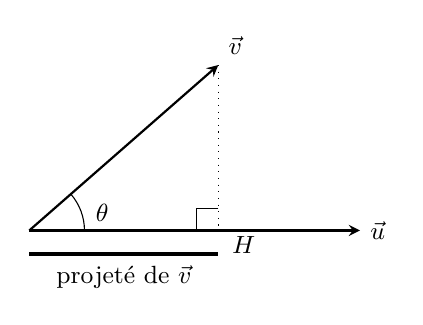
\begin{tikzpicture}[scale=1, >=stealth, every node/.style={font=\small}]
  \draw[->, thick] (0,0) -- (4.2,0) node[right] {$\vec u$};
  \draw[->, thick] (0,0) -- (2.4,2.1) node[above right] {$\vec v$};
  \draw[dotted] (2.4,2.1) -- (2.4,0);
  \draw (2.4,0.28) -- (2.12,0.28) -- (2.12,0);
  \draw[very thick] (0,-0.3) -- (2.4,-0.3);
  \node[below] at (1.2,-0.32) {projeté de $\vec v$};
  \draw (0.7,0) arc (0:41:0.7);
  \node[right] at (0.72,0.22) {$\theta$};
  \node[below right] at (2.45,0.05) {$H$};
\end{tikzpicture}
